\documentclass{article}
\usepackage{tikz}
\usepackage{amsmath}
\usepackage{caption}

\begin{document}

    \begin{figure}[ht]
        \centering
        \captionsetup{type=figure} % 不显示标题
        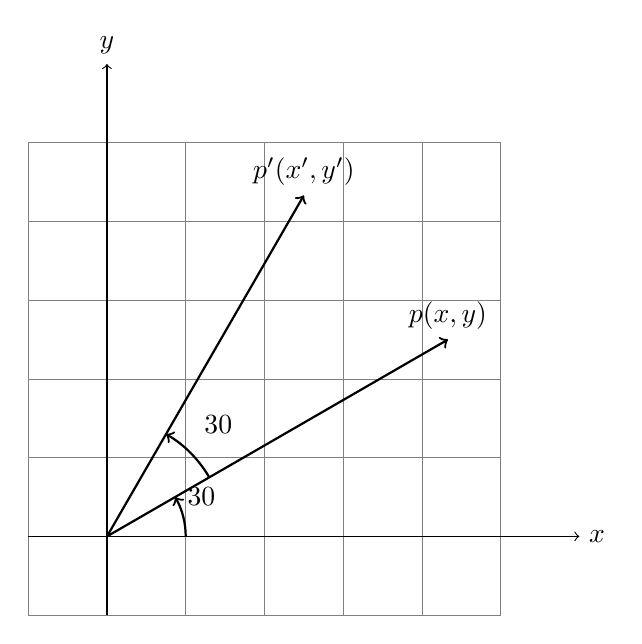
\begin{tikzpicture}
            \draw[very thin, gray] (-1,-1) grid (5,5);

            % 绘制坐标系
            \draw[->] (-1,0) -- (6,0) node[right] {$x$};
            \draw[->] (0,-1) -- (0,6) node[above] {$y$};

            % 计算初始线段和旋转后的线段的坐标
            \pgfmathsetmacro{\length}{5} % 线段长度
            \pgfmathsetmacro{\alpha}{30} % 初始角度
            \pgfmathsetmacro{\beta}{30} % 线段之间的夹角

            \pgfmathsetmacro{\x}{\length * cos(\alpha)} % 初始线段 x 坐标
            \pgfmathsetmacro{\y}{\length * sin(\alpha)} % 初始线段 y 坐标

            \pgfmathsetmacro{\xprime}{\length * cos(\alpha + \beta)} % 旋转后线段 x 坐标
            \pgfmathsetmacro{\yprime}{\length * sin(\alpha + \beta)} % 旋转后线段 y 坐标

            % 绘制初始线段和旋转后的线段
            \draw[->, thick] (0,0) -- (\x, \y);
            \draw[->, thick] (0,0) -- (\xprime, \yprime);

            % 标记角度
            \draw[->, thick] (1,0) arc[start angle=0,end angle=\alpha,radius=1cm];
            \node at (1.2,0.5) {$\alpha$};

            \draw[->, thick] (\alpha:1.5) arc[start angle=\alpha,end angle=\alpha+\beta,radius=1.5cm];
            \node at (\alpha+0.5*\beta:2) {$\beta$};

            % 标记长度
            \node at (\x, \y + 0.3) {$p(x, y)$};;
            \node at (\xprime, \yprime + 0.3) {$p'(x', y')$};;
        \end{tikzpicture}
        \caption*{} % 不显示标题
        \label{fig:figure} % 不显示标题
    \end{figure}

\end{document}
